\documentclass[1p]{elsarticle_modified}
%\bibliographystyle{elsarticle-num}

%\usepackage[colorlinks]{hyperref}
%\usepackage{abbrmath_seonhwa} %\Abb, \Ascr, \Acal ,\Abf, \Afrak
\usepackage{amsfonts}
\usepackage{amssymb}
\usepackage{amsmath}
\usepackage{amsthm}
\usepackage{scalefnt}
\usepackage{amsbsy}
\usepackage{kotex}
\usepackage{caption}
\usepackage{subfig}
\usepackage{color}
\usepackage{graphicx}
\usepackage{xcolor} %% white, black, red, green, blue, cyan, magenta, yellow
\usepackage{float}
\usepackage{setspace}
\usepackage{hyperref}

\usepackage{tikz}
\usetikzlibrary{arrows}

\usepackage{multirow}
\usepackage{array} % fixed length table
\usepackage{hhline}

%%%%%%%%%%%%%%%%%%%%%
\makeatletter
\renewcommand*\env@matrix[1][\arraystretch]{%
	\edef\arraystretch{#1}%
	\hskip -\arraycolsep
	\let\@ifnextchar\new@ifnextchar
	\array{*\c@MaxMatrixCols c}}
\makeatother %https://tex.stackexchange.com/questions/14071/how-can-i-increase-the-line-spacing-in-a-matrix
%%%%%%%%%%%%%%%

\usepackage[normalem]{ulem}

\newcommand{\msout}[1]{\ifmmode\text{\sout{\ensuremath{#1}}}\else\sout{#1}\fi}
%SOURCE: \msout is \stkout macro in https://tex.stackexchange.com/questions/20609/strikeout-in-math-mode

\newcommand{\cancel}[1]{
	\ifmmode
	{\color{red}\msout{#1}}
	\else
	{\color{red}\sout{#1}}
	\fi
}

\newcommand{\add}[1]{
	{\color{blue}\uwave{#1}}
}

\newcommand{\replace}[2]{
	\ifmmode
	{\color{red}\msout{#1}}{\color{blue}\uwave{#2}}
	\else
	{\color{red}\sout{#1}}{\color{blue}\uwave{#2}}
	\fi
}

\newcommand{\Sol}{\mathcal{S}} %segment
\newcommand{\D}{D} %diagram
\newcommand{\A}{\mathcal{A}} %arc


%%%%%%%%%%%%%%%%%%%%%%%%%%%%%5 test

\def\sl{\operatorname{\textup{SL}}(2,\Cbb)}
\def\psl{\operatorname{\textup{PSL}}(2,\Cbb)}
\def\quan{\mkern 1mu \triangleright \mkern 1mu}

\theoremstyle{definition}
\newtheorem{thm}{Theorem}[section]
\newtheorem{prop}[thm]{Proposition}
\newtheorem{lem}[thm]{Lemma}
\newtheorem{ques}[thm]{Question}
\newtheorem{cor}[thm]{Corollary}
\newtheorem{defn}[thm]{Definition}
\newtheorem{exam}[thm]{Example}
\newtheorem{rmk}[thm]{Remark}
\newtheorem{alg}[thm]{Algorithm}

\newcommand{\I}{\sqrt{-1}}
\begin{document}

%\begin{frontmatter}
%
%\title{Boundary parabolic representations of knots up to 8 crossings}
%
%%% Group authors per affiliation:
%\author{Yunhi Cho} 
%\address{Department of Mathematics, University of Seoul, Seoul, Korea}
%\ead{yhcho@uos.ac.kr}
%
%
%\author{Seonhwa Kim} %\fnref{s_kim}}
%\address{Center for Geometry and Physics, Institute for Basic Science, Pohang, 37673, Korea}
%\ead{ryeona17@ibs.re.kr}
%
%\author{Hyuk Kim}
%\address{Department of Mathematical Sciences, Seoul National University, Seoul 08826, Korea}
%\ead{hyukkim@snu.ac.kr}
%
%\author{Seokbeom Yoon}
%\address{Department of Mathematical Sciences, Seoul National University, Seoul, 08826,  Korea}
%\ead{sbyoon15@snu.ac.kr}
%
%\begin{abstract}
%We find all boundary parabolic representation of knots up to 8 crossings.
%
%\end{abstract}
%\begin{keyword}
%    \MSC[2010] 57M25 
%\end{keyword}
%
%\end{frontmatter}

%\linenumbers
%\tableofcontents
%
\newcommand\colored[1]{\textcolor{white}{\rule[-0.35ex]{0.8em}{1.4ex}}\kern-0.8em\color{red} #1}%
%\newcommand\colored[1]{\textcolor{white}{ #1}\kern-2.17ex	\textcolor{white}{ #1}\kern-1.81ex	\textcolor{white}{ #1}\kern-2.15ex\color{red}#1	}

{\Large $\underline{12a_{1114}~(K12a_{1114})}$}

\setlength{\tabcolsep}{10pt}
\renewcommand{\arraystretch}{1.6}
\vspace{1cm}\begin{tabular}{m{100pt}>{\centering\arraybackslash}m{274pt}}
\multirow{5}{120pt}{
	\centering
	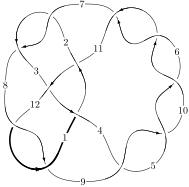
\includegraphics[width=112pt]{../../../GIT/diagram.site/Diagrams/png/1915_12a_1114.png}\\
\ \ \ A knot diagram\footnotemark}&
\allowdisplaybreaks
\textbf{Linearized knot diagam} \\
\cline{2-2}
 &
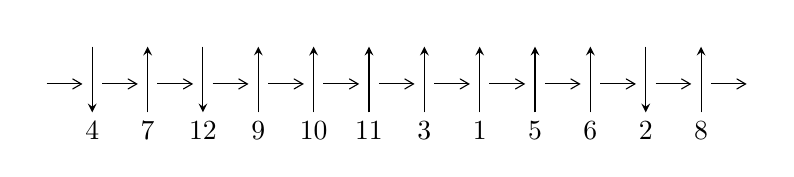
\begin{tikzpicture}[x=20pt, y=17pt]
	% nodes
	\node (C0) at (0, 0) {};
	\node (C1) at (1, 0) {};
	\node (C1U) at (1, +1) {};
	\node (C1D) at (1, -1) {4};

	\node (C2) at (2, 0) {};
	\node (C2U) at (2, +1) {};
	\node (C2D) at (2, -1) {7};

	\node (C3) at (3, 0) {};
	\node (C3U) at (3, +1) {};
	\node (C3D) at (3, -1) {12};

	\node (C4) at (4, 0) {};
	\node (C4U) at (4, +1) {};
	\node (C4D) at (4, -1) {9};

	\node (C5) at (5, 0) {};
	\node (C5U) at (5, +1) {};
	\node (C5D) at (5, -1) {10};

	\node (C6) at (6, 0) {};
	\node (C6U) at (6, +1) {};
	\node (C6D) at (6, -1) {11};

	\node (C7) at (7, 0) {};
	\node (C7U) at (7, +1) {};
	\node (C7D) at (7, -1) {3};

	\node (C8) at (8, 0) {};
	\node (C8U) at (8, +1) {};
	\node (C8D) at (8, -1) {1};

	\node (C9) at (9, 0) {};
	\node (C9U) at (9, +1) {};
	\node (C9D) at (9, -1) {5};

	\node (C10) at (10, 0) {};
	\node (C10U) at (10, +1) {};
	\node (C10D) at (10, -1) {6};

	\node (C11) at (11, 0) {};
	\node (C11U) at (11, +1) {};
	\node (C11D) at (11, -1) {2};

	\node (C12) at (12, 0) {};
	\node (C12U) at (12, +1) {};
	\node (C12D) at (12, -1) {8};
	\node (C13) at (13, 0) {};

	% arrows
	\draw[->,>={angle 60}]
	(C0) edge (C1) (C1) edge (C2) (C2) edge (C3) (C3) edge (C4) (C4) edge (C5) (C5) edge (C6) (C6) edge (C7) (C7) edge (C8) (C8) edge (C9) (C9) edge (C10) (C10) edge (C11) (C11) edge (C12) (C12) edge (C13) ;	\draw[->,>=stealth]
	(C1U) edge (C1D) (C2D) edge (C2U) (C3U) edge (C3D) (C4D) edge (C4U) (C5D) edge (C5U) (C6D) edge (C6U) (C7D) edge (C7U) (C8D) edge (C8U) (C9D) edge (C9U) (C10D) edge (C10U) (C11U) edge (C11D) (C12D) edge (C12U) ;
	\end{tikzpicture} \\
\hhline{~~} \\& 
\textbf{Solving Sequence} \\ \cline{2-2} 
 &
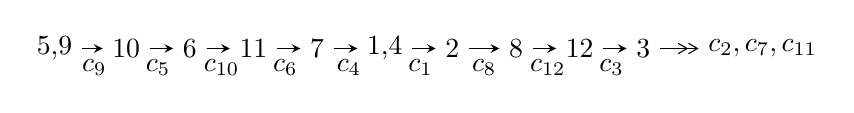
\begin{tikzpicture}[x=23pt, y=7pt]
	% node
	\node (A0) at (-1/8, 0) {5,9};
	\node (A1) at (1, 0) {10};
	\node (A2) at (2, 0) {6};
	\node (A3) at (3, 0) {11};
	\node (A4) at (4, 0) {7};
	\node (A5) at (81/16, 0) {1,4};
	\node (A6) at (49/8, 0) {2};
	\node (A7) at (57/8, 0) {8};
	\node (A8) at (65/8, 0) {12};
	\node (A9) at (73/8, 0) {3};
	\node (C1) at (1/2, -1) {$c_{9}$};
	\node (C2) at (3/2, -1) {$c_{5}$};
	\node (C3) at (5/2, -1) {$c_{10}$};
	\node (C4) at (7/2, -1) {$c_{6}$};
	\node (C5) at (9/2, -1) {$c_{4}$};
	\node (C6) at (45/8, -1) {$c_{1}$};
	\node (C7) at (53/8, -1) {$c_{8}$};
	\node (C8) at (61/8, -1) {$c_{12}$};
	\node (C9) at (69/8, -1) {$c_{3}$};
	\node (A10) at (11, 0) {$c_{2},c_{7},c_{11}$};

	% edge
	\draw[->,>=stealth]	
	(A0) edge (A1) (A1) edge (A2) (A2) edge (A3) (A3) edge (A4) (A4) edge (A5) (A5) edge (A6) (A6) edge (A7) (A7) edge (A8) (A8) edge (A9) ;
	\draw[->>,>={angle 60}]	
	(A9) edge (A10);
\end{tikzpicture} \\ 

\end{tabular} \\

\footnotetext{
The image of knot diagram is generated by the software ``\textbf{Draw programme}" developed by Andrew Bartholomew(\url{http://www.layer8.co.uk/maths/draw/index.htm\#Running-draw}), where we modified some parts for our purpose(\url{https://github.com/CATsTAILs/LinksPainter}).
}\phantom \\ \newline 
\centering \textbf{Ideals for irreducible components\footnotemark of $X_{\text{par}}$} 
 
\begin{align*}
I^u_{1}&=\langle 
49 u^{21}-206 u^{20}+\cdots+2 b-110,\;-13 u^{21}+48 u^{20}+\cdots+4 a+12,\;u^{22}-6 u^{21}+\cdots-14 u+4\rangle \\
I^u_{2}&=\langle 
-17691 u^8 a^3+8540 u^8 a^2+\cdots+277099 a-169388,\;-2 u^8 a^3-4 u^8 a^2+\cdots-12 a+70,\\
\phantom{I^u_{2}}&\phantom{= \langle  }u^9+u^8-6 u^7-5 u^6+11 u^5+7 u^4-6 u^3-4 u^2- u+1\rangle \\
I^u_{3}&=\langle 
u^4-3 u^2+b+1,\;u^7-6 u^5- u^4+11 u^3+3 u^2+a-6 u-1,\\
\phantom{I^u_{3}}&\phantom{= \langle  }u^{11}- u^{10}-8 u^9+7 u^8+23 u^7-16 u^6-29 u^5+13 u^4+15 u^3-2 u^2- u-1\rangle \\
\\
\end{align*}
\raggedright * 3 irreducible components of $\dim_{\mathbb{C}}=0$, with total 69 representations.\\
\footnotetext{All coefficients of polynomials are rational numbers. But the coefficients are sometimes approximated in decimal forms when there is not enough margin.}
\newpage
\renewcommand{\arraystretch}{1}
\centering \section*{I. $I^u_{1}= \langle 49 u^{21}-206 u^{20}+\cdots+2 b-110,\;-13 u^{21}+48 u^{20}+\cdots+4 a+12,\;u^{22}-6 u^{21}+\cdots-14 u+4 \rangle$}
\flushleft \textbf{(i) Arc colorings}\\
\begin{tabular}{m{7pt} m{180pt} m{7pt} m{180pt} }
\flushright $a_{5}=$&$\begin{pmatrix}0\\u\end{pmatrix}$ \\
\flushright $a_{9}=$&$\begin{pmatrix}1\\0\end{pmatrix}$ \\
\flushright $a_{10}=$&$\begin{pmatrix}1\\- u^2\end{pmatrix}$ \\
\flushright $a_{6}=$&$\begin{pmatrix}u\\- u^3+u\end{pmatrix}$ \\
\flushright $a_{11}=$&$\begin{pmatrix}- u^2+1\\u^4-2 u^2\end{pmatrix}$ \\
\flushright $a_{7}=$&$\begin{pmatrix}- u^3+2 u\\u^5-3 u^3+u\end{pmatrix}$ \\
\flushright $a_{1}=$&$\begin{pmatrix}\frac{13}{4} u^{21}-12 u^{20}+\cdots+\frac{51}{4} u-3\\-\frac{49}{2} u^{21}+103 u^{20}+\cdots-\frac{323}{2} u+55\end{pmatrix}$ \\
\flushright $a_{4}=$&$\begin{pmatrix}- u\\u\end{pmatrix}$ \\
\flushright $a_{2}=$&$\begin{pmatrix}\frac{265}{4} u^{21}-281 u^{20}+\cdots+\frac{1755}{4} u-149\\-\frac{175}{2} u^{21}+372 u^{20}+\cdots-\frac{1175}{2} u+201\end{pmatrix}$ \\
\flushright $a_{8}=$&$\begin{pmatrix}\frac{1}{2} u^{21}-\frac{1}{2} u^{20}+\cdots-\frac{5}{2} u+\frac{3}{2}\\-\frac{17}{2} u^{21}+35 u^{20}+\cdots-\frac{109}{2} u+18\end{pmatrix}$ \\
\flushright $a_{12}=$&$\begin{pmatrix}19 u^{21}-\frac{163}{2} u^{20}+\cdots+127 u-\frac{85}{2}\\-\frac{45}{2} u^{21}+97 u^{20}+\cdots-\frac{313}{2} u+54\end{pmatrix}$ \\
\flushright $a_{3}=$&$\begin{pmatrix}\frac{49}{4} u^{21}-54 u^{20}+\cdots+\frac{339}{4} u-29\\-\frac{23}{2} u^{21}+52 u^{20}+\cdots-\frac{175}{2} u+31\end{pmatrix}$\\&\end{tabular}
\flushleft \textbf{(ii) Obstruction class $= -1$}\\~\\
\flushleft \textbf{(iii) Cusp Shapes $= -42 u^{21}+180 u^{20}+180 u^{19}-1614 u^{18}+357 u^{17}+6114 u^{16}-4208 u^{15}-12099 u^{14}+13221 u^{13}+11109 u^{12}-22235 u^{11}+1566 u^{10}+20908 u^9-13794 u^8-7898 u^7+12460 u^6-2905 u^5-4228 u^4+2792 u^3+18 u^2-316 u+106$}\\~\\
\newpage\renewcommand{\arraystretch}{1}
\flushleft \textbf{(iv) u-Polynomials at the component}\newline \\
\begin{tabular}{m{50pt}|m{274pt}}
Crossings & \hspace{64pt}u-Polynomials at each crossing \\
\hline $$\begin{aligned}c_{1},c_{11}\end{aligned}$$&$\begin{aligned}
&u^{22}+2 u^{21}+\cdots-12 u+1
\end{aligned}$\\
\hline $$\begin{aligned}c_{2},c_{7},c_{8}\\c_{12}\end{aligned}$$&$\begin{aligned}
&u^{22}+u^{21}+\cdots-2 u+1
\end{aligned}$\\
\hline $$\begin{aligned}c_{3}\end{aligned}$$&$\begin{aligned}
&u^{22}+21 u^{21}+\cdots+2816 u+512
\end{aligned}$\\
\hline $$\begin{aligned}c_{4},c_{5},c_{6}\\c_{9},c_{10}\end{aligned}$$&$\begin{aligned}
&u^{22}+6 u^{21}+\cdots+14 u+4
\end{aligned}$\\
\hline
\end{tabular}\\~\\
\newpage\renewcommand{\arraystretch}{1}
\flushleft \textbf{(v) Riley Polynomials at the component}\newline \\
\begin{tabular}{m{50pt}|m{274pt}}
Crossings & \hspace{64pt}Riley Polynomials at each crossing \\
\hline $$\begin{aligned}c_{1},c_{11}\end{aligned}$$&$\begin{aligned}
&y^{22}+14 y^{21}+\cdots-162 y+1
\end{aligned}$\\
\hline $$\begin{aligned}c_{2},c_{7},c_{8}\\c_{12}\end{aligned}$$&$\begin{aligned}
&y^{22}-21 y^{21}+\cdots-10 y+1
\end{aligned}$\\
\hline $$\begin{aligned}c_{3}\end{aligned}$$&$\begin{aligned}
&y^{22}- y^{21}+\cdots-7405568 y+262144
\end{aligned}$\\
\hline $$\begin{aligned}c_{4},c_{5},c_{6}\\c_{9},c_{10}\end{aligned}$$&$\begin{aligned}
&y^{22}-30 y^{21}+\cdots-140 y+16
\end{aligned}$\\
\hline
\end{tabular}\\~\\
\newpage\flushleft \textbf{(vi) Complex Volumes and Cusp Shapes}
$$\begin{array}{c|c|c}  
\text{Solutions to }I^u_{1}& \I (\text{vol} + \sqrt{-1}CS) & \text{Cusp shape}\\
 \hline 
\begin{aligned}
u &= -1.043890 + 0.084239 I \\
a &= -0.396837 - 0.057037 I \\
b &= \phantom{-}0.016671 - 0.768015 I\end{aligned}
 & \phantom{-}2.64990 - 1.99958 I & \phantom{-}9.53146 + 3.76378 I \\ \hline\begin{aligned}
u &= -1.043890 - 0.084239 I \\
a &= -0.396837 + 0.057037 I \\
b &= \phantom{-}0.016671 + 0.768015 I\end{aligned}
 & \phantom{-}2.64990 + 1.99958 I & \phantom{-}9.53146 - 3.76378 I \\ \hline\begin{aligned}
u &= \phantom{-}0.319390 + 0.784311 I \\
a &= \phantom{-}0.105537 - 0.519872 I \\
b &= -1.332750 + 0.209642 I\end{aligned}
 & \phantom{-}6.57558 - 3.17716 I & \phantom{-}14.5871 + 2.3802 I \\ \hline\begin{aligned}
u &= \phantom{-}0.319390 - 0.784311 I \\
a &= \phantom{-}0.105537 + 0.519872 I \\
b &= -1.332750 - 0.209642 I\end{aligned}
 & \phantom{-}6.57558 + 3.17716 I & \phantom{-}14.5871 - 2.3802 I \\ \hline\begin{aligned}
u &= \phantom{-}0.495362 + 0.681217 I \\
a &= -0.623279 + 1.001900 I \\
b &= \phantom{-}1.38604 + 0.33811 I\end{aligned}
 & \phantom{-}7.16423 + 7.89598 I & \phantom{-}13.0600 - 7.3152 I \\ \hline\begin{aligned}
u &= \phantom{-}0.495362 - 0.681217 I \\
a &= -0.623279 - 1.001900 I \\
b &= \phantom{-}1.38604 - 0.33811 I\end{aligned}
 & \phantom{-}7.16423 - 7.89598 I & \phantom{-}13.0600 + 7.3152 I \\ \hline\begin{aligned}
u &= -1.220570 + 0.357902 I \\
a &= \phantom{-}1.81374 + 0.84055 I \\
b &= -1.48578 + 0.42742 I\end{aligned}
 & \phantom{-}12.5903 - 11.4735 I & \phantom{-}15.1438 + 6.9415 I \\ \hline\begin{aligned}
u &= -1.220570 - 0.357902 I \\
a &= \phantom{-}1.81374 - 0.84055 I \\
b &= -1.48578 - 0.42742 I\end{aligned}
 & \phantom{-}12.5903 + 11.4735 I & \phantom{-}15.1438 - 6.9415 I \\ \hline\begin{aligned}
u &= -1.193250 + 0.493321 I \\
a &= -1.23495 - 0.92705 I \\
b &= \phantom{-}1.339160 + 0.061996 I\end{aligned}
 & \phantom{-}11.24460 - 1.24294 I & \phantom{-}18.1099 + 1.8376 I \\ \hline\begin{aligned}
u &= -1.193250 - 0.493321 I \\
a &= -1.23495 + 0.92705 I \\
b &= \phantom{-}1.339160 - 0.061996 I\end{aligned}
 & \phantom{-}11.24460 + 1.24294 I & \phantom{-}18.1099 - 1.8376 I\\
 \hline 
 \end{array}$$\newpage$$\begin{array}{c|c|c}  
\text{Solutions to }I^u_{1}& \I (\text{vol} + \sqrt{-1}CS) & \text{Cusp shape}\\
 \hline 
\begin{aligned}
u &= \phantom{-}0.687446\phantom{ +0.000000I} \\
a &= \phantom{-}2.18879\phantom{ +0.000000I} \\
b &= -0.499542\phantom{ +0.000000I}\end{aligned}
 & -0.430924\phantom{ +0.000000I} & \phantom{-}21.8170\phantom{ +0.000000I} \\ \hline\begin{aligned}
u &= \phantom{-}1.48411\phantom{ +0.000000I} \\
a &= -0.786366\phantom{ +0.000000I} \\
b &= \phantom{-}0.649714\phantom{ +0.000000I}\end{aligned}
 & \phantom{-}6.96114\phantom{ +0.000000I} & \phantom{-}19.0070\phantom{ +0.000000I} \\ \hline\begin{aligned}
u &= -0.411824\phantom{ +0.000000I} \\
a &= \phantom{-}0.523537\phantom{ +0.000000I} \\
b &= -0.318922\phantom{ +0.000000I}\end{aligned}
 & \phantom{-}0.605966\phantom{ +0.000000I} & \phantom{-}16.6960\phantom{ +0.000000I} \\ \hline\begin{aligned}
u &= -1.58824\phantom{ +0.000000I} \\
a &= -1.60194\phantom{ +0.000000I} \\
b &= \phantom{-}0.874121\phantom{ +0.000000I}\end{aligned}
 & \phantom{-}7.51930\phantom{ +0.000000I} & \phantom{-}14.0920\phantom{ +0.000000I} \\ \hline\begin{aligned}
u &= \phantom{-}0.227373 + 0.272091 I \\
a &= \phantom{-}0.53987 - 1.57107 I \\
b &= \phantom{-}0.082959 - 0.502394 I\end{aligned}
 & -1.28640 + 0.84268 I & -1.69920 - 4.23368 I \\ \hline\begin{aligned}
u &= \phantom{-}0.227373 - 0.272091 I \\
a &= \phantom{-}0.53987 + 1.57107 I \\
b &= \phantom{-}0.082959 + 0.502394 I\end{aligned}
 & -1.28640 - 0.84268 I & -1.69920 + 4.23368 I \\ \hline\begin{aligned}
u &= \phantom{-}1.74549 + 0.01514 I \\
a &= \phantom{-}0.268462 + 0.256545 I \\
b &= -0.047072 - 0.943997 I\end{aligned}
 & \phantom{-}12.75810 + 2.36846 I & \phantom{-}10.71272 - 2.85205 I \\ \hline\begin{aligned}
u &= \phantom{-}1.74549 - 0.01514 I \\
a &= \phantom{-}0.268462 - 0.256545 I \\
b &= -0.047072 + 0.943997 I\end{aligned}
 & \phantom{-}12.75810 - 2.36846 I & \phantom{-}10.71272 + 2.85205 I \\ \hline\begin{aligned}
u &= \phantom{-}1.78669 + 0.09389 I \\
a &= -2.11796 + 0.46248 I \\
b &= \phantom{-}1.56385 + 0.48092 I\end{aligned}
 & -16.0394 + 13.4812 I & \phantom{-}15.5774 - 5.8403 I \\ \hline\begin{aligned}
u &= \phantom{-}1.78669 - 0.09389 I \\
a &= -2.11796 - 0.46248 I \\
b &= \phantom{-}1.56385 - 0.48092 I\end{aligned}
 & -16.0394 - 13.4812 I & \phantom{-}15.5774 + 5.8403 I\\
 \hline 
 \end{array}$$\newpage$$\begin{array}{c|c|c}  
\text{Solutions to }I^u_{1}& \I (\text{vol} + \sqrt{-1}CS) & \text{Cusp shape}\\
 \hline 
\begin{aligned}
u &= \phantom{-}1.79765 + 0.12560 I \\
a &= \phantom{-}1.73341 - 0.61996 I \\
b &= -1.375760 - 0.072217 I\end{aligned}
 & -17.4882 + 3.9741 I & \phantom{-}17.1708 - 2.2051 I \\ \hline\begin{aligned}
u &= \phantom{-}1.79765 - 0.12560 I \\
a &= \phantom{-}1.73341 + 0.61996 I \\
b &= -1.375760 + 0.072217 I\end{aligned}
 & -17.4882 - 3.9741 I & \phantom{-}17.1708 + 2.2051 I\\
 \hline 
 \end{array}$$\newpage\newpage\renewcommand{\arraystretch}{1}
\centering \section*{II. $I^u_{2}= \langle -1.77\times10^{4} a^{3} u^{8}+8540 a^{2} u^{8}+\cdots+2.77\times10^{5} a-1.69\times10^{5},\;-2 u^8 a^3-4 u^8 a^2+\cdots-12 a+70,\;u^9+u^8+\cdots- u+1 \rangle$}
\flushleft \textbf{(i) Arc colorings}\\
\begin{tabular}{m{7pt} m{180pt} m{7pt} m{180pt} }
\flushright $a_{5}=$&$\begin{pmatrix}0\\u\end{pmatrix}$ \\
\flushright $a_{9}=$&$\begin{pmatrix}1\\0\end{pmatrix}$ \\
\flushright $a_{10}=$&$\begin{pmatrix}1\\- u^2\end{pmatrix}$ \\
\flushright $a_{6}=$&$\begin{pmatrix}u\\- u^3+u\end{pmatrix}$ \\
\flushright $a_{11}=$&$\begin{pmatrix}- u^2+1\\u^4-2 u^2\end{pmatrix}$ \\
\flushright $a_{7}=$&$\begin{pmatrix}- u^3+2 u\\u^5-3 u^3+u\end{pmatrix}$ \\
\flushright $a_{1}=$&$\begin{pmatrix}a\\0.0802571 a^{3} u^{8}-0.0387426 a^{2} u^{8}+\cdots-1.25709 a+0.768447\end{pmatrix}$ \\
\flushright $a_{4}=$&$\begin{pmatrix}- u\\u\end{pmatrix}$ \\
\flushright $a_{2}=$&$\begin{pmatrix}-0.709439 a^{3} u^{8}+0.329072 a^{2} u^{8}+\cdots+2.30427 a-1.91298\\0.789696 a^{3} u^{8}-0.367815 a^{2} u^{8}+\cdots-2.56136 a+2.68143\end{pmatrix}$ \\
\flushright $a_{8}=$&$\begin{pmatrix}-0.307278 a^{3} u^{8}+0.496604 a^{2} u^{8}+\cdots-0.507896 a-2.73403\\0.428369 a^{3} u^{8}+0.0229598 a^{2} u^{8}+\cdots+0.390062 a+3.89304\end{pmatrix}$ \\
\flushright $a_{12}=$&$\begin{pmatrix}0.229521 a^{3} u^{8}-0.705855 a^{2} u^{8}+\cdots+0.724728 a+3.72904\\-0.441407 a^{3} u^{8}+2.28443 a^{2} u^{8}+\cdots-3.25779 a-5.21324\end{pmatrix}$ \\
\flushright $a_{3}=$&$\begin{pmatrix}-0.946141 a^{3} u^{8}-0.800857 a^{2} u^{8}+\cdots+1.80509 a-3.49748\\1.15803 a^{3} u^{8}-0.777715 a^{2} u^{8}+\cdots+0.727971 a+3.98169\end{pmatrix}$\\&\end{tabular}
\flushleft \textbf{(ii) Obstruction class $= -1$}\\~\\
\flushleft \textbf{(iii) Cusp Shapes $= -\frac{31188}{20039} u^8 a^3-\frac{18668}{20039} u^8 a^2+\cdots+\frac{7244}{20039} a+\frac{311386}{20039}$}\\~\\
\newpage\renewcommand{\arraystretch}{1}
\flushleft \textbf{(iv) u-Polynomials at the component}\newline \\
\begin{tabular}{m{50pt}|m{274pt}}
Crossings & \hspace{64pt}u-Polynomials at each crossing \\
\hline $$\begin{aligned}c_{1},c_{11}\end{aligned}$$&$\begin{aligned}
&u^{36}-11 u^{35}+\cdots-22476 u+2977
\end{aligned}$\\
\hline $$\begin{aligned}c_{2},c_{7},c_{8}\\c_{12}\end{aligned}$$&$\begin{aligned}
&u^{36}- u^{35}+\cdots-12 u+1
\end{aligned}$\\
\hline $$\begin{aligned}c_{3}\end{aligned}$$&$\begin{aligned}
&(u^2- u+1)^{18}
\end{aligned}$\\
\hline $$\begin{aligned}c_{4},c_{5},c_{6}\\c_{9},c_{10}\end{aligned}$$&$\begin{aligned}
&(u^9- u^8-6 u^7+5 u^6+11 u^5-7 u^4-6 u^3+4 u^2- u-1)^4
\end{aligned}$\\
\hline
\end{tabular}\\~\\
\newpage\renewcommand{\arraystretch}{1}
\flushleft \textbf{(v) Riley Polynomials at the component}\newline \\
\begin{tabular}{m{50pt}|m{274pt}}
Crossings & \hspace{64pt}Riley Polynomials at each crossing \\
\hline $$\begin{aligned}c_{1},c_{11}\end{aligned}$$&$\begin{aligned}
&y^{36}+19 y^{35}+\cdots+113199956 y+8862529
\end{aligned}$\\
\hline $$\begin{aligned}c_{2},c_{7},c_{8}\\c_{12}\end{aligned}$$&$\begin{aligned}
&y^{36}-33 y^{35}+\cdots+13206 y^2+1
\end{aligned}$\\
\hline $$\begin{aligned}c_{3}\end{aligned}$$&$\begin{aligned}
&(y^2+y+1)^{18}
\end{aligned}$\\
\hline $$\begin{aligned}c_{4},c_{5},c_{6}\\c_{9},c_{10}\end{aligned}$$&$\begin{aligned}
&(y^9-13 y^8+68 y^7-183 y^6+269 y^5-211 y^4+80 y^3-18 y^2+9 y-1)^{4}
\end{aligned}$\\
\hline
\end{tabular}\\~\\
\newpage\flushleft \textbf{(vi) Complex Volumes and Cusp Shapes}
$$\begin{array}{c|c|c}  
\text{Solutions to }I^u_{2}& \I (\text{vol} + \sqrt{-1}CS) & \text{Cusp shape}\\
 \hline 
\begin{aligned}
u &= \phantom{-}1.115700 + 0.218357 I \\
a &= -0.583676 - 0.658151 I \\
b &= -0.0692851 + 0.0614982 I\end{aligned}
 & \phantom{-}6.69287 + 1.83365 I & \phantom{-}14.03791 - 0.54536 I \\ \hline\begin{aligned}
u &= \phantom{-}1.115700 + 0.218357 I \\
a &= -0.648434 - 0.438924 I \\
b &= \phantom{-}0.381836 + 1.212390 I\end{aligned}
 & \phantom{-}6.69287 + 5.89342 I & \phantom{-}14.0379 - 7.4736 I \\ \hline\begin{aligned}
u &= \phantom{-}1.115700 + 0.218357 I \\
a &= -1.48443 + 0.60451 I \\
b &= \phantom{-}1.294760 + 0.266822 I\end{aligned}
 & \phantom{-}6.69287 + 1.83365 I & \phantom{-}14.03791 - 0.54536 I \\ \hline\begin{aligned}
u &= \phantom{-}1.115700 + 0.218357 I \\
a &= \phantom{-}1.72894 - 1.32529 I \\
b &= -1.278910 - 0.315259 I\end{aligned}
 & \phantom{-}6.69287 + 5.89342 I & \phantom{-}14.0379 - 7.4736 I \\ \hline\begin{aligned}
u &= \phantom{-}1.115700 - 0.218357 I \\
a &= -0.583676 + 0.658151 I \\
b &= -0.0692851 - 0.0614982 I\end{aligned}
 & \phantom{-}6.69287 - 1.83365 I & \phantom{-}14.03791 + 0.54536 I \\ \hline\begin{aligned}
u &= \phantom{-}1.115700 - 0.218357 I \\
a &= -0.648434 + 0.438924 I \\
b &= \phantom{-}0.381836 - 1.212390 I\end{aligned}
 & \phantom{-}6.69287 - 5.89342 I & \phantom{-}14.0379 + 7.4736 I \\ \hline\begin{aligned}
u &= \phantom{-}1.115700 - 0.218357 I \\
a &= -1.48443 - 0.60451 I \\
b &= \phantom{-}1.294760 - 0.266822 I\end{aligned}
 & \phantom{-}6.69287 - 1.83365 I & \phantom{-}14.03791 + 0.54536 I \\ \hline\begin{aligned}
u &= \phantom{-}1.115700 - 0.218357 I \\
a &= \phantom{-}1.72894 + 1.32529 I \\
b &= -1.278910 + 0.315259 I\end{aligned}
 & \phantom{-}6.69287 - 5.89342 I & \phantom{-}14.0379 + 7.4736 I \\ \hline\begin{aligned}
u &= -1.15527\phantom{ +0.000000I} \\
a &= -2.01543 + 0.07577 I \\
b &= \phantom{-}1.63501 + 0.66222 I\end{aligned}
 & \phantom{-}10.43600 + 2.02988 I & \phantom{-}18.5753 - 3.4641 I \\ \hline\begin{aligned}
u &= -1.15527\phantom{ +0.000000I} \\
a &= -2.01543 - 0.07577 I \\
b &= \phantom{-}1.63501 - 0.66222 I\end{aligned}
 & \phantom{-}10.43600 - 2.02988 I & \phantom{-}18.5753 + 3.4641 I\\
 \hline 
 \end{array}$$\newpage$$\begin{array}{c|c|c}  
\text{Solutions to }I^u_{2}& \I (\text{vol} + \sqrt{-1}CS) & \text{Cusp shape}\\
 \hline 
\begin{aligned}
u &= -1.15527\phantom{ +0.000000I} \\
a &= \phantom{-}2.74857 + 1.19407 I \\
b &= -1.263110 - 0.018083 I\end{aligned}
 & \phantom{-}10.43600 + 2.02988 I & \phantom{-}18.5753 - 3.4641 I \\ \hline\begin{aligned}
u &= -1.15527\phantom{ +0.000000I} \\
a &= \phantom{-}2.74857 - 1.19407 I \\
b &= -1.263110 + 0.018083 I\end{aligned}
 & \phantom{-}10.43600 - 2.02988 I & \phantom{-}18.5753 + 3.4641 I \\ \hline\begin{aligned}
u &= -0.344156 + 0.466288 I \\
a &= -0.231060 + 0.764559 I \\
b &= -1.169060 - 0.018719 I\end{aligned}
 & \phantom{-}2.08691 + 0.47566 I & \phantom{-}8.94040 + 0.84117 I \\ \hline\begin{aligned}
u &= -0.344156 + 0.466288 I \\
a &= \phantom{-}1.310650 - 0.167710 I \\
b &= \phantom{-}0.082806 + 0.524016 I\end{aligned}
 & \phantom{-}2.08691 + 0.47566 I & \phantom{-}8.94040 + 0.84117 I \\ \hline\begin{aligned}
u &= -0.344156 + 0.466288 I \\
a &= \phantom{-}0.032067 + 0.569438 I \\
b &= -0.222763 + 0.891266 I\end{aligned}
 & \phantom{-}2.08691 - 3.58411 I & \phantom{-}8.94040 + 7.76937 I \\ \hline\begin{aligned}
u &= -0.344156 + 0.466288 I \\
a &= -0.05497 - 1.80281 I \\
b &= \phantom{-}1.203490 - 0.203190 I\end{aligned}
 & \phantom{-}2.08691 - 3.58411 I & \phantom{-}8.94040 + 7.76937 I \\ \hline\begin{aligned}
u &= -0.344156 - 0.466288 I \\
a &= -0.231060 - 0.764559 I \\
b &= -1.169060 + 0.018719 I\end{aligned}
 & \phantom{-}2.08691 - 0.47566 I & \phantom{-}8.94040 - 0.84117 I \\ \hline\begin{aligned}
u &= -0.344156 - 0.466288 I \\
a &= \phantom{-}1.310650 + 0.167710 I \\
b &= \phantom{-}0.082806 - 0.524016 I\end{aligned}
 & \phantom{-}2.08691 - 0.47566 I & \phantom{-}8.94040 - 0.84117 I \\ \hline\begin{aligned}
u &= -0.344156 - 0.466288 I \\
a &= \phantom{-}0.032067 - 0.569438 I \\
b &= -0.222763 - 0.891266 I\end{aligned}
 & \phantom{-}2.08691 + 3.58411 I & \phantom{-}8.94040 - 7.76937 I \\ \hline\begin{aligned}
u &= -0.344156 - 0.466288 I \\
a &= -0.05497 + 1.80281 I \\
b &= \phantom{-}1.203490 + 0.203190 I\end{aligned}
 & \phantom{-}2.08691 + 3.58411 I & \phantom{-}8.94040 - 7.76937 I\\
 \hline 
 \end{array}$$\newpage$$\begin{array}{c|c|c}  
\text{Solutions to }I^u_{2}& \I (\text{vol} + \sqrt{-1}CS) & \text{Cusp shape}\\
 \hline 
\begin{aligned}
u &= \phantom{-}0.362481\phantom{ +0.000000I} \\
a &= \phantom{-}1.11687 + 1.72823 I \\
b &= -1.38930 + 0.48183 I\end{aligned}
 & \phantom{-}5.49604 - 2.02988 I & \phantom{-}19.6128 + 3.4641 I \\ \hline\begin{aligned}
u &= \phantom{-}0.362481\phantom{ +0.000000I} \\
a &= \phantom{-}1.11687 - 1.72823 I \\
b &= -1.38930 - 0.48183 I\end{aligned}
 & \phantom{-}5.49604 + 2.02988 I & \phantom{-}19.6128 - 3.4641 I \\ \hline\begin{aligned}
u &= \phantom{-}0.362481\phantom{ +0.000000I} \\
a &= -3.85979 + 3.02264 I \\
b &= \phantom{-}1.225600 - 0.198299 I\end{aligned}
 & \phantom{-}5.49604 - 2.02988 I & \phantom{-}19.6128 + 3.4641 I \\ \hline\begin{aligned}
u &= \phantom{-}0.362481\phantom{ +0.000000I} \\
a &= -3.85979 - 3.02264 I \\
b &= \phantom{-}1.225600 + 0.198299 I\end{aligned}
 & \phantom{-}5.49604 + 2.02988 I & \phantom{-}19.6128 - 3.4641 I \\ \hline\begin{aligned}
u &= -1.76115 + 0.05266 I \\
a &= \phantom{-}0.634605 - 0.837704 I \\
b &= -0.43558 + 1.42750 I\end{aligned}
 & \phantom{-}17.1037 - 7.0247 I & \phantom{-}14.8663 + 6.3722 I \\ \hline\begin{aligned}
u &= -1.76115 + 0.05266 I \\
a &= \phantom{-}0.263385 - 0.472901 I \\
b &= \phantom{-}0.086713 - 0.200842 I\end{aligned}
 & \phantom{-}17.1037 - 2.9650 I & \phantom{-}14.8663 - 0.5560 I \\ \hline\begin{aligned}
u &= -1.76115 + 0.05266 I \\
a &= \phantom{-}1.82935 + 0.17038 I \\
b &= -1.43895 + 0.44937 I\end{aligned}
 & \phantom{-}17.1037 - 2.9650 I & \phantom{-}14.8663 - 0.5560 I \\ \hline\begin{aligned}
u &= -1.76115 + 0.05266 I \\
a &= -1.94297 - 0.82339 I \\
b &= \phantom{-}1.326930 - 0.380702 I\end{aligned}
 & \phantom{-}17.1037 - 7.0247 I & \phantom{-}14.8663 + 6.3722 I \\ \hline\begin{aligned}
u &= -1.76115 - 0.05266 I \\
a &= \phantom{-}0.634605 + 0.837704 I \\
b &= -0.43558 - 1.42750 I\end{aligned}
 & \phantom{-}17.1037 + 7.0247 I & \phantom{-}14.8663 - 6.3722 I \\ \hline\begin{aligned}
u &= -1.76115 - 0.05266 I \\
a &= \phantom{-}0.263385 + 0.472901 I \\
b &= \phantom{-}0.086713 + 0.200842 I\end{aligned}
 & \phantom{-}17.1037 + 2.9650 I & \phantom{-}14.8663 + 0.5560 I\\
 \hline 
 \end{array}$$\newpage$$\begin{array}{c|c|c}  
\text{Solutions to }I^u_{2}& \I (\text{vol} + \sqrt{-1}CS) & \text{Cusp shape}\\
 \hline 
\begin{aligned}
u &= -1.76115 - 0.05266 I \\
a &= \phantom{-}1.82935 - 0.17038 I \\
b &= -1.43895 - 0.44937 I\end{aligned}
 & \phantom{-}17.1037 + 2.9650 I & \phantom{-}14.8663 + 0.5560 I \\ \hline\begin{aligned}
u &= -1.76115 - 0.05266 I \\
a &= -1.94297 + 0.82339 I \\
b &= \phantom{-}1.326930 + 0.380702 I\end{aligned}
 & \phantom{-}17.1037 + 7.0247 I & \phantom{-}14.8663 - 6.3722 I \\ \hline\begin{aligned}
u &= \phantom{-}1.77199\phantom{ +0.000000I} \\
a &= \phantom{-}2.19492 + 0.22581 I \\
b &= -1.78129 - 0.74916 I\end{aligned}
 & -18.3509 + 2.0299 I & \phantom{-}18.1228 - 3.4641 I \\ \hline\begin{aligned}
u &= \phantom{-}1.77199\phantom{ +0.000000I} \\
a &= \phantom{-}2.19492 - 0.22581 I \\
b &= -1.78129 + 0.74916 I\end{aligned}
 & -18.3509 - 2.0299 I & \phantom{-}18.1228 + 3.4641 I \\ \hline\begin{aligned}
u &= \phantom{-}1.77199\phantom{ +0.000000I} \\
a &= -2.53859 + 0.82107 I \\
b &= \phantom{-}1.311100 + 0.065235 I\end{aligned}
 & -18.3509 - 2.0299 I & \phantom{-}18.1228 + 3.4641 I \\ \hline\begin{aligned}
u &= \phantom{-}1.77199\phantom{ +0.000000I} \\
a &= -2.53859 - 0.82107 I \\
b &= \phantom{-}1.311100 - 0.065235 I\end{aligned}
 & -18.3509 + 2.0299 I & \phantom{-}18.1228 - 3.4641 I\\
 \hline 
 \end{array}$$\newpage\newpage\renewcommand{\arraystretch}{1}
\centering \section*{III. $I^u_{3}= \langle u^4-3 u^2+b+1,\;u^7-6 u^5- u^4+11 u^3+3 u^2+a-6 u-1,\;u^{11}- u^{10}+\cdots- u-1 \rangle$}
\flushleft \textbf{(i) Arc colorings}\\
\begin{tabular}{m{7pt} m{180pt} m{7pt} m{180pt} }
\flushright $a_{5}=$&$\begin{pmatrix}0\\u\end{pmatrix}$ \\
\flushright $a_{9}=$&$\begin{pmatrix}1\\0\end{pmatrix}$ \\
\flushright $a_{10}=$&$\begin{pmatrix}1\\- u^2\end{pmatrix}$ \\
\flushright $a_{6}=$&$\begin{pmatrix}u\\- u^3+u\end{pmatrix}$ \\
\flushright $a_{11}=$&$\begin{pmatrix}- u^2+1\\u^4-2 u^2\end{pmatrix}$ \\
\flushright $a_{7}=$&$\begin{pmatrix}- u^3+2 u\\u^5-3 u^3+u\end{pmatrix}$ \\
\flushright $a_{1}=$&$\begin{pmatrix}- u^7+6 u^5+u^4-11 u^3-3 u^2+6 u+1\\- u^4+3 u^2-1\end{pmatrix}$ \\
\flushright $a_{4}=$&$\begin{pmatrix}- u\\u\end{pmatrix}$ \\
\flushright $a_{2}=$&$\begin{pmatrix}u^9-7 u^7+17 u^5+u^4-17 u^3-3 u^2+6 u+1\\- u^9+6 u^7-11 u^5- u^4+6 u^3+3 u^2-1\end{pmatrix}$ \\
\flushright $a_{8}=$&$\begin{pmatrix}u^{10}- u^9-8 u^8+7 u^7+22 u^6-16 u^5-24 u^4+14 u^3+8 u^2-5 u+1\\u^8-6 u^6+11 u^4-6 u^2+1\end{pmatrix}$ \\
\flushright $a_{12}=$&$\begin{pmatrix}- u^9+7 u^7-16 u^5+13 u^3- u^2-2 u+2\\u^9-7 u^7+16 u^5+u^4-13 u^3-3 u^2+2 u+1\end{pmatrix}$ \\
\flushright $a_{3}=$&$\begin{pmatrix}u^9-8 u^7+22 u^5+u^4-24 u^3-3 u^2+8 u+1\\- u^4+3 u^2+u-1\end{pmatrix}$\\&\end{tabular}
\flushleft \textbf{(ii) Obstruction class $= 1$}\\~\\
\flushleft \textbf{(iii) Cusp Shapes $= -4 u^{10}+2 u^9+31 u^8-14 u^7-82 u^6+27 u^5+84 u^4-6 u^3-23 u^2-10 u+5$}\\~\\
\newpage\renewcommand{\arraystretch}{1}
\flushleft \textbf{(iv) u-Polynomials at the component}\newline \\
\begin{tabular}{m{50pt}|m{274pt}}
Crossings & \hspace{64pt}u-Polynomials at each crossing \\
\hline $$\begin{aligned}c_{1},c_{11}\end{aligned}$$&$\begin{aligned}
&u^{11}+2 u^{10}+3 u^9+4 u^8+u^7-2 u^6-5 u^5-5 u^4-2 u^3+u^2+2 u+1
\end{aligned}$\\
\hline $$\begin{aligned}c_{2},c_{8}\end{aligned}$$&$\begin{aligned}
&u^{11}+u^{10}+\cdots-4 u-1
\end{aligned}$\\
\hline $$\begin{aligned}c_{3}\end{aligned}$$&$\begin{aligned}
&u^{11}-2 u^{10}+u^9+2 u^8-5 u^7+5 u^6-2 u^5- u^4+4 u^3-3 u^2+2 u-1
\end{aligned}$\\
\hline $$\begin{aligned}c_{4},c_{5},c_{6}\end{aligned}$$&$\begin{aligned}
&u^{11}+u^{10}+\cdots- u+1
\end{aligned}$\\
\hline $$\begin{aligned}c_{7},c_{12}\end{aligned}$$&$\begin{aligned}
&u^{11}- u^{10}+\cdots-4 u+1
\end{aligned}$\\
\hline $$\begin{aligned}c_{9},c_{10}\end{aligned}$$&$\begin{aligned}
&u^{11}- u^{10}+\cdots- u-1
\end{aligned}$\\
\hline
\end{tabular}\\~\\
\newpage\renewcommand{\arraystretch}{1}
\flushleft \textbf{(v) Riley Polynomials at the component}\newline \\
\begin{tabular}{m{50pt}|m{274pt}}
Crossings & \hspace{64pt}Riley Polynomials at each crossing \\
\hline $$\begin{aligned}c_{1},c_{11}\end{aligned}$$&$\begin{aligned}
&y^{11}+2 y^{10}-5 y^9-12 y^8+3 y^7+14 y^6+y^5-5 y^4-2 y^3+y^2+2 y-1
\end{aligned}$\\
\hline $$\begin{aligned}c_{2},c_{7},c_{8}\\c_{12}\end{aligned}$$&$\begin{aligned}
&y^{11}-13 y^{10}+\cdots+38 y-1
\end{aligned}$\\
\hline $$\begin{aligned}c_{3}\end{aligned}$$&$\begin{aligned}
&y^{11}-2 y^{10}- y^9+2 y^8+5 y^7- y^6-14 y^5-3 y^4+12 y^3+5 y^2-2 y-1
\end{aligned}$\\
\hline $$\begin{aligned}c_{4},c_{5},c_{6}\\c_{9},c_{10}\end{aligned}$$&$\begin{aligned}
&y^{11}-17 y^{10}+\cdots-3 y-1
\end{aligned}$\\
\hline
\end{tabular}\\~\\
\newpage\flushleft \textbf{(vi) Complex Volumes and Cusp Shapes}
$$\begin{array}{c|c|c}  
\text{Solutions to }I^u_{3}& \I (\text{vol} + \sqrt{-1}CS) & \text{Cusp shape}\\
 \hline 
\begin{aligned}
u &= -1.003860 + 0.215654 I \\
a &= -0.834543 - 0.532608 I \\
b &= \phantom{-}1.147190 - 0.466546 I\end{aligned}
 & \phantom{-}7.60023 - 3.64229 I & \phantom{-}16.7867 + 4.7032 I \\ \hline\begin{aligned}
u &= -1.003860 - 0.215654 I \\
a &= -0.834543 + 0.532608 I \\
b &= \phantom{-}1.147190 + 0.466546 I\end{aligned}
 & \phantom{-}7.60023 + 3.64229 I & \phantom{-}16.7867 - 4.7032 I \\ \hline\begin{aligned}
u &= \phantom{-}1.288880 + 0.118905 I \\
a &= -1.87499 + 0.32616 I \\
b &= \phantom{-}1.322320 - 0.090164 I\end{aligned}
 & \phantom{-}9.54739 - 0.09465 I & \phantom{-}15.9387 + 0.1893 I \\ \hline\begin{aligned}
u &= \phantom{-}1.288880 - 0.118905 I \\
a &= -1.87499 - 0.32616 I \\
b &= \phantom{-}1.322320 + 0.090164 I\end{aligned}
 & \phantom{-}9.54739 + 0.09465 I & \phantom{-}15.9387 - 0.1893 I \\ \hline\begin{aligned}
u &= \phantom{-}0.550251\phantom{ +0.000000I} \\
a &= \phantom{-}1.93961\phantom{ +0.000000I} \\
b &= -0.183345\phantom{ +0.000000I}\end{aligned}
 & -0.771716\phantom{ +0.000000I} & -1.63370\phantom{ +0.000000I} \\ \hline\begin{aligned}
u &= -1.53837\phantom{ +0.000000I} \\
a &= -0.987197\phantom{ +0.000000I} \\
b &= \phantom{-}0.499049\phantom{ +0.000000I}\end{aligned}
 & \phantom{-}6.40308\phantom{ +0.000000I} & \phantom{-}3.17420\phantom{ +0.000000I} \\ \hline\begin{aligned}
u &= -0.146441 + 0.318421 I \\
a &= -0.12310 + 2.31687 I \\
b &= -1.237540 - 0.294692 I\end{aligned}
 & \phantom{-}4.72595 + 1.79241 I & \phantom{-}7.60505 + 0.27412 I \\ \hline\begin{aligned}
u &= -0.146441 - 0.318421 I \\
a &= -0.12310 - 2.31687 I \\
b &= -1.237540 + 0.294692 I\end{aligned}
 & \phantom{-}4.72595 - 1.79241 I & \phantom{-}7.60505 - 0.27412 I \\ \hline\begin{aligned}
u &= \phantom{-}1.74679 + 0.05665 I \\
a &= \phantom{-}1.167540 - 0.166105 I \\
b &= -1.107360 - 0.612780 I\end{aligned}
 & \phantom{-}17.5808 + 4.7820 I & \phantom{-}16.4667 - 3.6309 I \\ \hline\begin{aligned}
u &= \phantom{-}1.74679 - 0.05665 I \\
a &= \phantom{-}1.167540 + 0.166105 I \\
b &= -1.107360 + 0.612780 I\end{aligned}
 & \phantom{-}17.5808 - 4.7820 I & \phantom{-}16.4667 + 3.6309 I\\
 \hline 
 \end{array}$$\newpage$$\begin{array}{c|c|c}  
\text{Solutions to }I^u_{3}& \I (\text{vol} + \sqrt{-1}CS) & \text{Cusp shape}\\
 \hline 
\begin{aligned}
u &= -1.78263\phantom{ +0.000000I} \\
a &= \phantom{-}2.37775\phantom{ +0.000000I} \\
b &= -1.56492\phantom{ +0.000000I}\end{aligned}
 & -18.7427\phantom{ +0.000000I} & \phantom{-}16.8650\phantom{ +0.000000I}\\
 \hline 
 \end{array}$$\newpage
\newpage\renewcommand{\arraystretch}{1}
\centering \section*{ IV. u-Polynomials}
\begin{tabular}{m{50pt}|m{274pt}}
Crossings & \hspace{64pt}u-Polynomials at each crossing \\
\hline $$\begin{aligned}c_{1},c_{11}\end{aligned}$$&$\begin{aligned}
&(u^{11}+2 u^{10}+3 u^9+4 u^8+u^7-2 u^6-5 u^5-5 u^4-2 u^3+u^2+2 u+1)\\
&\cdot(u^{22}+2 u^{21}+\cdots-12 u+1)(u^{36}-11 u^{35}+\cdots-22476 u+2977)
\end{aligned}$\\
\hline $$\begin{aligned}c_{2},c_{8}\end{aligned}$$&$\begin{aligned}
&(u^{11}+u^{10}+\cdots-4 u-1)(u^{22}+u^{21}+\cdots-2 u+1)\\
&\cdot(u^{36}- u^{35}+\cdots-12 u+1)
\end{aligned}$\\
\hline $$\begin{aligned}c_{3}\end{aligned}$$&$\begin{aligned}
&(u^2- u+1)^{18}\\
&\cdot(u^{11}-2 u^{10}+u^9+2 u^8-5 u^7+5 u^6-2 u^5- u^4+4 u^3-3 u^2+2 u-1)\\
&\cdot(u^{22}+21 u^{21}+\cdots+2816 u+512)
\end{aligned}$\\
\hline $$\begin{aligned}c_{4},c_{5},c_{6}\end{aligned}$$&$\begin{aligned}
&(u^9- u^8-6 u^7+5 u^6+11 u^5-7 u^4-6 u^3+4 u^2- u-1)^4\\
&\cdot(u^{11}+u^{10}+\cdots- u+1)(u^{22}+6 u^{21}+\cdots+14 u+4)
\end{aligned}$\\
\hline $$\begin{aligned}c_{7},c_{12}\end{aligned}$$&$\begin{aligned}
&(u^{11}- u^{10}+\cdots-4 u+1)(u^{22}+u^{21}+\cdots-2 u+1)\\
&\cdot(u^{36}- u^{35}+\cdots-12 u+1)
\end{aligned}$\\
\hline $$\begin{aligned}c_{9},c_{10}\end{aligned}$$&$\begin{aligned}
&(u^9- u^8-6 u^7+5 u^6+11 u^5-7 u^4-6 u^3+4 u^2- u-1)^4\\
&\cdot(u^{11}- u^{10}+\cdots- u-1)(u^{22}+6 u^{21}+\cdots+14 u+4)
\end{aligned}$\\
\hline
\end{tabular}\newpage\renewcommand{\arraystretch}{1}
\centering \section*{ V. Riley Polynomials}
\begin{tabular}{m{50pt}|m{274pt}}
Crossings & \hspace{64pt}Riley Polynomials at each crossing \\
\hline $$\begin{aligned}c_{1},c_{11}\end{aligned}$$&$\begin{aligned}
&(y^{11}+2 y^{10}-5 y^9-12 y^8+3 y^7+14 y^6+y^5-5 y^4-2 y^3+y^2+2 y-1)\\
&\cdot(y^{22}+14 y^{21}+\cdots-162 y+1)\\
&\cdot(y^{36}+19 y^{35}+\cdots+113199956 y+8862529)
\end{aligned}$\\
\hline $$\begin{aligned}c_{2},c_{7},c_{8}\\c_{12}\end{aligned}$$&$\begin{aligned}
&(y^{11}-13 y^{10}+\cdots+38 y-1)(y^{22}-21 y^{21}+\cdots-10 y+1)\\
&\cdot(y^{36}-33 y^{35}+\cdots+13206 y^2+1)
\end{aligned}$\\
\hline $$\begin{aligned}c_{3}\end{aligned}$$&$\begin{aligned}
&(y^2+y+1)^{18}\\
&\cdot(y^{11}-2 y^{10}- y^9+2 y^8+5 y^7- y^6-14 y^5-3 y^4+12 y^3+5 y^2-2 y-1)\\
&\cdot(y^{22}- y^{21}+\cdots-7405568 y+262144)
\end{aligned}$\\
\hline $$\begin{aligned}c_{4},c_{5},c_{6}\\c_{9},c_{10}\end{aligned}$$&$\begin{aligned}
&(y^9-13 y^8+68 y^7-183 y^6+269 y^5-211 y^4+80 y^3-18 y^2+9 y-1)^{4}\\
&\cdot(y^{11}-17 y^{10}+\cdots-3 y-1)(y^{22}-30 y^{21}+\cdots-140 y+16)
\end{aligned}$\\
\hline
\end{tabular}
\vskip 2pc
\end{document}